\pdfminorversion=4 % for acroread
%\documentclass[aspectratio=169,t,xcolor={usenames,dvipsnames}]{beamer}
\documentclass[aspectratio=169,t,handout,xcolor={usenames,dvipsnames}]{beamer}
\usepackage{../beamerstyle}
\usepackage{dsfont}
\usepackage{bm}
\usepackage[english]{babel}
\usepackage[utf8]{inputenc}
\usepackage{graphicx}
\usepackage{algorithm}
\usepackage[ruled,vlined,algo2e,linesnumbered]{algorithm2e}
%\usepackage[boxed,vlined]{algorithm2e}
\usepackage{hyperref}
\usepackage{booktabs}
\usepackage{mathtools}

\usepackage{amsmath,amssymb}
\usepackage{listings}
\lstset{frame=lines,framesep=3pt,numbers=left,numberblanklines=false,basicstyle=\ttfamily\small}

\usepackage{subfig}
\usepackage{multicol}
%\usepackage{appendixnumberbeamer}
%
\usepackage{tcolorbox}

\usepackage{pgfplots}
\usepackage{tikz}
\usetikzlibrary{trees} 
\usetikzlibrary{shapes.geometric}
\usetikzlibrary{positioning,shapes,shadows,arrows,calc,mindmap}
\usetikzlibrary{positioning,fadings,through}
\usetikzlibrary{decorations.pathreplacing}
\usetikzlibrary{intersections}
\usetikzlibrary{positioning,fit,calc,shadows,backgrounds}
\pgfdeclarelayer{background}
\pgfdeclarelayer{foreground}
\pgfsetlayers{background,main,foreground}
\tikzstyle{activity}=[rectangle, draw=black, rounded corners, text centered, text width=8em]
\tikzstyle{data}=[rectangle, draw=black, text centered, text width=8em]
\tikzstyle{myarrow}=[->, thick, draw=black]

% Define the layers to draw the diagram
\pgfdeclarelayer{background}
\pgfdeclarelayer{foreground}
\pgfsetlayers{background,main,foreground}

%\usepackage{listings}
%\lstset{numbers=left,
%  showstringspaces=false,
%  frame={tb},
%  captionpos=b,
%  lineskip=0pt,
%  basicstyle=\ttfamily,
%%  extendedchars=true,
%  stepnumber=1,
%  numberstyle=\small,
%  xleftmargin=1em,
%  breaklines
%}

 
\definecolor{blue}{RGB}{0, 74, 153}

\usetheme{Boadilla}
%\useinnertheme{rectangles}
\usecolortheme{whale}
\setbeamercolor{alerted text}{fg=blue}
\useoutertheme{infolines}
\setbeamertemplate{navigation symbols}{\vspace{-5pt}} % to lower the logo
\setbeamercolor{date in head/foot}{bg=white} % blue
\setbeamercolor{date in head/foot}{fg=white}
\setbeamercolor{author  in head/foot}{bg=white} %blue
\setbeamercolor{title in head/foot}{bg=white} % blue
\setbeamercolor{title}{fg=white, bg=blue}
\setbeamercolor{block title}{fg=white,bg=blue}
\setbeamercolor{block body}{bg=blue!10}
\setbeamercolor{frametitle}{fg=white, bg=blue}
\setbeamercovered{invisible}

\makeatletter
\setbeamertemplate{footline}
{
  \leavevmode%
  \hbox{%
  \begin{beamercolorbox}[wd=.333333\paperwidth,ht=2.25ex,dp=1ex,center]{author in head/foot}%
%    \usebeamerfont{author in head/foot}\insertshortauthor
  \end{beamercolorbox}%
  \begin{beamercolorbox}[wd=.333333\paperwidth,ht=2.25ex,dp=1ex,center]{title in head/foot}%
    \usebeamerfont{title in head/foot}\insertshorttitle
  \end{beamercolorbox}%
  \begin{beamercolorbox}[wd=.333333\paperwidth,ht=2.25ex,dp=1ex,right]{date in head/foot}%
    \usebeamerfont{date in head/foot}\insertshortdate{}\hspace*{2em}
%    \insertframenumber\hspace*{2ex} 
  \end{beamercolorbox}}%
  \vskip0pt%
}
\makeatother

%\pgfdeclareimage[height=1.2cm]{automl}{images/logos/automl.png}
%\pgfdeclareimage[height=1.2cm]{freiburg}{images/logos/freiburg}

%\logo{\pgfuseimage{freiburg}}

\renewcommand{\comment}[1]{
	\noindent
	%\vspace{0.25cm}
	{\color{red}{\textbf{TODO:} #1}}
	%\vspace{0.25cm}
}
\newcommand{\notefh}[1]{\textcolor{red}{\textbf{FH:} #1}}
\renewcommand{\comment}[1]{}
\newcommand{\hide}[1]{}
\newcommand{\cemph}[2]{\emph{\textcolor{#1}{#2}}}

\newcommand{\lit}[1]{{\footnotesize\color{black!60}[#1]}}

\newcommand{\litw}[1]{{\footnotesize\color{blue!20}[#1]}}


\newcommand{\myframe}[2]{\begin{frame}[c]{#1}#2\end{frame}}
\newcommand{\myframetop}[2]{\begin{frame}{#1}#2\end{frame}}
\newcommand{\myit}[1]{\begin{itemize}#1\end{itemize}}
\newcommand{\myblock}[2]{\begin{block}{#1}#2\end{block}}


\newcommand{\votepurple}[1]{\textcolor{Purple}{$\bigstar$}}
\newcommand{\voteyellow}[1]{\textcolor{Goldenrod}{$\bigstar$}}
\newcommand{\voteblue}[1]{\textcolor{RoyalBlue}{$\bigstar$}}
\newcommand{\votepink}[1]{\textcolor{Pink}{$\bigstar$}}

\newcommand{\diff}{\mathop{}\!\mathrm{d}}
\newcommand{\refstyle}[1]{{\small{\textcolor{gray}{#1}}}}
\newcommand{\hands}[0]{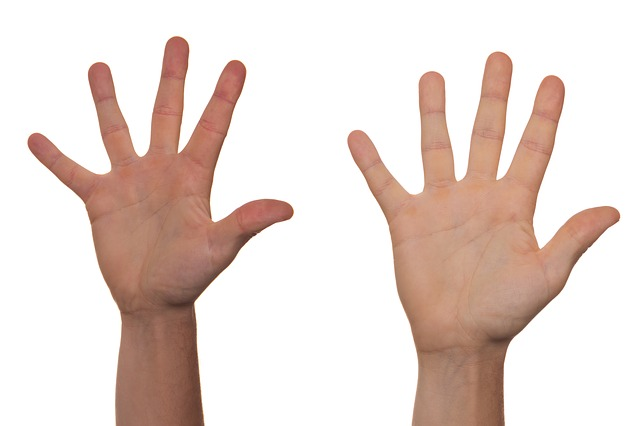
\includegraphics[height=1.5em]{images/hands}}
\newcommand{\transpose}[0]{{\textrm{\tiny{\sf{T}}}}}
\newcommand{\norm}{{\mathcal{N}}}
\newcommand{\cutoff}[0]{\kappa}
\newcommand{\instD}[0]{\dataset}
\newcommand{\insts}[0]{\mathcal{I}}
\newcommand{\inst}[0]{i}
\newcommand{\instI}[1]{i^{(#1)}}

% Iteration specific instance of variable/function/anything
% Introduced in the BO section, but moved up here to make it available within other macros
\newcommand{\iter}[2][\bocount]{{#2}^{(#1)}}

%--------HPO parameter macros-----------

% Parameter Configuration Space
\newcommand{\pcs}[0]{\pmb{\Lambda}}

% ???
\newcommand{\bx}[0]{\conf}

% Parameter Configuration
\newcommand{\conf}[0]{\pmb{\lambda}}

% Final Configuration
\newcommand{\finconf}[0]{\pmb{\hat{\lambda}}}

% Configuration corresponding to a given iteration -- better use \iter!
\newcommand{\confI}[1]{{\conf}^{(#1)}}

% Default Configuration
\newcommand{\defconf}[0]{{\conf}_{\text{def}}}

% Incumbent Configuration
\newcommand{\incumbent}[1][\bocount]{\iter[#1]{\finconf}}

% Optimal Configuration
\newcommand{\optconf}[0]{{\conf}^*}

% Configuration Space
\newcommand{\confs}[0]{\pcs}

%----------------------------------------

%\newcommand{\vlambda}[0]{\bm{\lambda}}
%\newcommand{\vLambda}[0]{\bm{\Lambda}}
\newcommand{\dataset}[0]{\mathcal{D}}
\newcommand{\datasets}[0]{\mathbf{D}}
\newcommand{\loss}[0]{L}
\newcommand{\risk}{\mathcal{R}}
\newcommand{\riske}{\mathcal{R}_{\text{emp}}}
\newcommand{\cost}[0]{c}
\newcommand{\costI}[1]{c^{(#1)}}

% Gaussian Process
\newcommand{\gp}{\mathcal{G}}
% Family of Objective Functions
\newcommand{\objF}{F}

%---------------BO Macros------------------

% BO loop counter
\newcommand{\bocount}{t}
% BO loop counter max, the counter runs from 1 to this value
\newcommand{\bobudget}{T}
% BO loop observation
\newcommand{\obs}[1][\conf]{\cost({#1})}
% BO loop observation space
\newcommand{\obsspace}{\mathcal{Y}}
% BO loop next observation
\newcommand{\bonextobs}{\obs[\iter{\conf}]}
% Acquisition Function, no args
\newcommand{\acq}{u}
% Standard Normal PDF
\newcommand{\pdf}{\phi}
% Standard Normal CDF
\newcommand{\cdf}{\Phi}
% Mean
\newcommand{\mean}{\mu}
% Standard Deviation
\newcommand{\stddev}{\sigma}
% Variance
\newcommand{\variance}{\sigma^2}
% Noise
\newcommand{\noise}{\nu}
% BO loop next selected sample
\newcommand{\bonextsample}{\confI{\bocount}}

% Single hyperparameter
\newcommand{\hyperparam}{\lambda}

% Single hyperparameter within a hyperparameter configuration
\newcommand{\hyperparami}[1][i]{{\hyperparam}_#1}

% Full definition of final configuration
\newcommand{\finconffull}{\incumbent[\bobudget]}

% Dataset
\newcommand{\datasetHPO}{{\dataset}_{HPO}}

% Dataset definition
\newcommand{\datasetHPOdef}{{\langle \bonextsample,\,\bonextobs \rangle}_{\bocount=1}^{\bobudget}}

% Double Display Fraction, forces large displays for everything in numerator and denominator
\newcommand\ddfrac[2]{\frac{\displaystyle #1}{\displaystyle #2}}

% Conditional Probability "Given That" Relation, source:https://tex.stackexchange.com/a/141685/205886
\newcommand\given[1][]{\:#1\vert\:}

% Expectation as a math operator
\DeclareMathOperator*{\E}{\mathbb{E}}

% Citation 
\newcommand{\source}[1]{
    \begin{flushright}
    	Source: \lit{#1}
    \end{flushright}
}
%-------------------------------------------

%Real numbers set
\newcommand{\realnum}{\mathbb{R}}
%Configuration space - do not use
%\newcommand{\configspace}{\Theta}
%Instances - do not use
%\newcommand{\instances}{\mathcal{I}}
%Expected value
\newcommand{\expectation}{\mathbb{E}}
%Kernel
\newcommand{\kernel}{\kappa}
%Constraint function
\newcommand{\constraintf}{c}
%Normal distribution
\newcommand{\normaldist}{\mathcal{N}}

% \renewcommand{\vec}[1]{\mathbf{#1}}
\newcommand{\hist}[0]{\dataset_{\text{Hist}}}
\newcommand{\param}[0]{p}
\newcommand{\algo}[0]{\mathcal{A}}
\newcommand{\algos}[0]{\mathbf{A}}
%\newcommand{\nn}[0]{N}
\newcommand{\feats}[0]{\mathcal{X}_{\text{meta}}}
\newcommand{\feat}[0]{\x_{\text{meta}}}
%\newcommand{\cluster}[0]{\vec{h}}
%\newcommand{\clusters}[0]{\vec{H}}
\newcommand{\perf}[0]{\mathbb{R}}
%\newcommand{\surro}[0]{\mathcal{S}}
\newcommand{\surro}[0]{\hat{\cost}}
\newcommand{\func}[0]{f}
\newcommand{\epm}[0]{\surro}
\newcommand{\portfolio}[0]{\mathbf{P}}
\newcommand{\schedule}[0]{\mathcal{S}}

% Machine Learning
\newcommand{\mdata}[0]{\dataset_{\text{meta}}}
\newcommand{\datasettrain}[0]{\dataset_{\text{train}}}
\newcommand{\datasetval}[0]{\dataset_{\text{val}}}
\newcommand{\datasettest}[0]{\dataset_{\text{test}}}
\newcommand{\x}[0]{\mathbf{x}}
\newcommand{\y}[0]{y}
\newcommand{\xI}[1]{\mathbf{x}^{(#1)}}
\newcommand{\yI}[1]{y^{(#1)}}
\newcommand{\fx}{f(\mathbf{x})}  % f(x), continuous prediction function
\newcommand{\Hspace}{\mathcal{H}} % hypothesis space where f is from
\newcommand{\fh}{\hat{f}}       % f hat, estimated prediction function

% Deep Learning
\newcommand{\weights}[0]{\theta}
\newcommand{\metaweights}[0]{\phi}


% reinforcement learning
\newcommand{\policies}[0]{\mathbf{\Pi}}
\newcommand{\policy}[0]{\pi}
\newcommand{\actionRL}[0]{a}
\newcommand{\stateRL}[0]{s}
\newcommand{\statesRL}[0]{\mathcal{S}}
\newcommand{\rewardRL}[0]{r}
\newcommand{\rewardfuncRL}[0]{\mathcal{R}}

\RestyleAlgo{algoruled}
\DontPrintSemicolon
\LinesNumbered
\SetAlgoVlined
\SetFuncSty{textsc}

\SetKwInOut{Input}{Input}
\SetKwInOut{Output}{Output}
\SetKw{Return}{return}

%\newcommand{\changed}[1]{{\color{red}#1}}

%\newcommand{\citeN}[1]{\citeauthor{#1}~(\citeyear{#1})}

\renewcommand{\vec}[1]{\mathbf{#1}}
\DeclareMathOperator*{\argmin}{arg\,min}
\DeclareMathOperator*{\argmax}{arg\,max}

%\newcommand{\aqme}{\textit{AQME}}
%\newcommand{\aslib}{\textit{ASlib}}
%\newcommand{\llama}{\textit{LLAMA}}
%\newcommand{\satzilla}{\textit{SATzilla}}
%\newcommand{\satzillaY}[1]{\textit{SATzilla'{#1}}}
%\newcommand{\snnap}{\textit{SNNAP}}
%\newcommand{\claspfolioTwo}{\textit{claspfolio~2}}
%\newcommand{\flexfolio}{\textit{FlexFolio}}
%\newcommand{\claspfolioOne}{\textit{claspfolio~1}}
%\newcommand{\isac}{\textit{ISAC}}
%\newcommand{\eisac}{\textit{EISAC}}
%\newcommand{\sss}{\textit{3S}}
%\newcommand{\sunny}{\textit{Sunny}}
%\newcommand{\ssspar}{\textit{3Spar}}
%\newcommand{\cshc}{\textit{CSHC}}
%\newcommand{\cshcpar}{\textit{CSHCpar}}
%\newcommand{\measp}{\textit{ME-ASP}}
%\newcommand{\aspeed}{\textit{aspeed}}
%\newcommand{\autofolio}{\textit{AutoFolio}}
%\newcommand{\cedalion}{\textit{Cedalion}}
\newcommand{\fanova}{\textit{fANOVA}}
\newcommand{\sbs}{\textit{SB}}
\newcommand{\oracle}{\textit{VBS}}

% like approaches
\newcommand{\claspfoliolike}[1]{\texttt{claspfolio-#1-like}}
\newcommand{\satzillalike}[1]{\texttt{SATzilla'#1-like}}
\newcommand{\isaclike}{\texttt{ISAC-like}}
\newcommand{\ssslike}{\texttt{3S-like}}
\newcommand{\measplike}{\texttt{ME-ASP-like}}

\newcommand{\irace}{\textit{I/F-race}}
\newcommand{\gga}{\textit{GGA}}
\newcommand{\smac}{\textit{SMAC}}
\newcommand{\paramils}{\textit{ParamILS}}
\newcommand{\spearmint}{\textit{Spearmint}}
\newcommand{\tpe}{\textit{TPE}}


\usepackage{pifont}
\newcommand{\itarrow}{\mbox{\Pisymbol{pzd}{229}}}
\newcommand{\ithook}{\mbox{\Pisymbol{pzd}{52}}}
\newcommand{\itcross}{\mbox{\Pisymbol{pzd}{56}}}
\newcommand{\ithand}{\mbox{\raisebox{-1pt}{\Pisymbol{pzd}{43}}}}

%\DeclareMathOperator*{\argmax}{arg\,max}

\newcommand{\ie}{{\it{}i.e.\/}}
\newcommand{\eg}{{\it{}e.g.\/}}
\newcommand{\cf}{{\it{}cf.\/}}
\newcommand{\wrt}{\mbox{w.r.t.}}
\newcommand{\vs}{{\it{}vs\/}}
\newcommand{\vsp}{{\it{}vs\/}}
\newcommand{\etc}{{\copyedit{etc.}}}
\newcommand{\etal}{{\it{}et al.\/}}

\newcommand{\pscProc}{{\bf procedure}}
\newcommand{\pscBegin}{{\bf begin}}
\newcommand{\pscEnd}{{\bf end}}
\newcommand{\pscEndIf}{{\bf endif}}
\newcommand{\pscFor}{{\bf for}}
\newcommand{\pscEach}{{\bf each}}
\newcommand{\pscThen}{{\bf then}}
\newcommand{\pscElse}{{\bf else}}
\newcommand{\pscWhile}{{\bf while}}
\newcommand{\pscIf}{{\bf if}}
\newcommand{\pscRepeat}{{\bf repeat}}
\newcommand{\pscUntil}{{\bf until}}
\newcommand{\pscWithProb}{{\bf with probability}}
\newcommand{\pscOtherwise}{{\bf otherwise}}
\newcommand{\pscDo}{{\bf do}}
\newcommand{\pscTo}{{\bf to}}
\newcommand{\pscOr}{{\bf or}}
\newcommand{\pscAnd}{{\bf and}}
\newcommand{\pscNot}{{\bf not}}
\newcommand{\pscFalse}{{\bf false}}
\newcommand{\pscEachElOf}{{\bf each element of}}
\newcommand{\pscReturn}{{\bf return}}

%\newcommand{\param}[1]{{\sl{}#1}}
\newcommand{\var}[1]{{\it{}#1}}
\newcommand{\cond}[1]{{\sf{}#1}}
%\newcommand{\state}[1]{{\sf{}#1}}
%\newcommand{\func}[1]{{\sl{}#1}}
\newcommand{\set}[1]{{\Bbb #1}}
%\newcommand{\inst}[1]{{\tt{}#1}}
\newcommand{\myurl}[1]{{\small\sf #1}}

\newcommand{\Nats}{{\Bbb N}}
\newcommand{\Reals}{{\Bbb R}}
\newcommand{\extset}[2]{\{#1 \; | \; #2\}}

\newcommand{\vbar}{$\,\;|$\hspace*{-1em}\raisebox{-0.3mm}{$\,\;\;|$}}
\newcommand{\vendbar}{\raisebox{+0.4mm}{$\,\;|$}}
\newcommand{\vend}{$\,\:\lfloor$}


\newcommand{\goleft}[2][.7]{\parbox[t]{#1\linewidth}{\strut\raggedright #2\strut}}
\newcommand{\rightimage}[2][.3]{\mbox{}\hfill\raisebox{1em-\height}[0pt][0pt]{\includegraphics[width=#1\linewidth]{#2}}\vspace*{-\baselineskip}}






\title[AutoML: NAS]{AutoML: Neural Architecture Search (NAS)} 
\subtitle{The One-Shot Model}
\author[Marius Lindauer]{Bernd Bischl \and \underline{Frank Hutter} \and Lars Kotthoff\newline \and Marius Lindauer \and Joaquin Vanschoren}
\institute{}
\date{}

\begin{document}
\maketitle

%-------------------------------------------------
%-------------------------------------------------

%----------------------------------------------------------------------
\myframetop{One-shot models: convolutional neural fabrics \litw{\href{https://arxiv.org/pdf/1606.02492.pdf}{Saxena and Verbeek. 2017}}}{
	\myit{
		\item A \alert{one-shot model} is a big model that has all architectures in a search space as submodels
		\myit{
			\item This allows weights sharing across architectures
			\item One \alert{only needs to train the single one-shot model}, \\ and implicitly trains an exponential number of individual architectures
		}
	}
%\pause

%\bigskip
	\myit{
		\item The first type of one-shot models: \alert{convolutional neural fabrics} %/ \alert{lattice} 

	\centering
	\only<2-5>{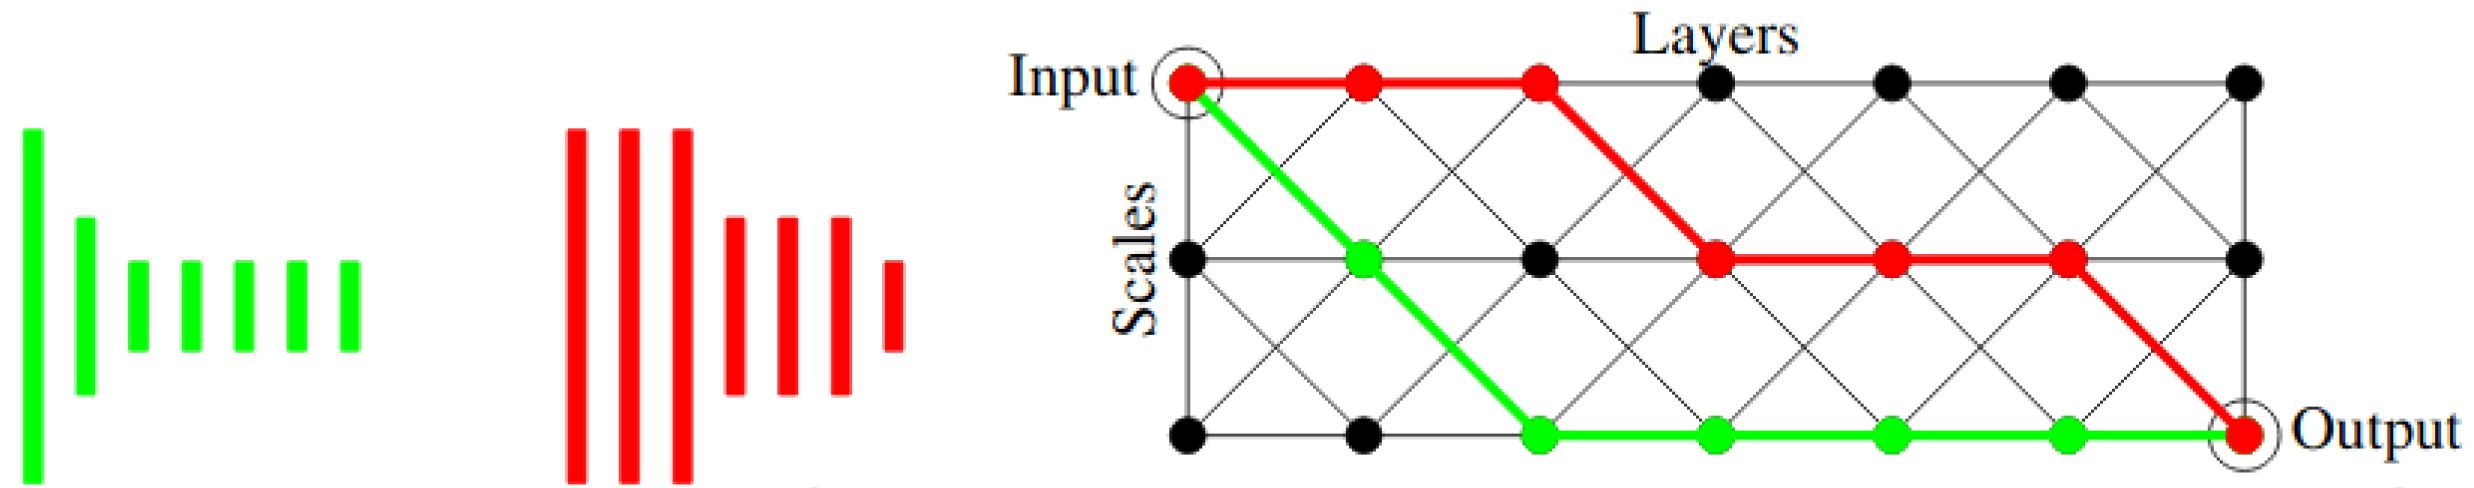
\includegraphics[width=0.7\textwidth]{images/conv_fabric_1.jpg}\\}
	%\only<6>{\hspace*{-0.91cm}\vspace*{0.3cm}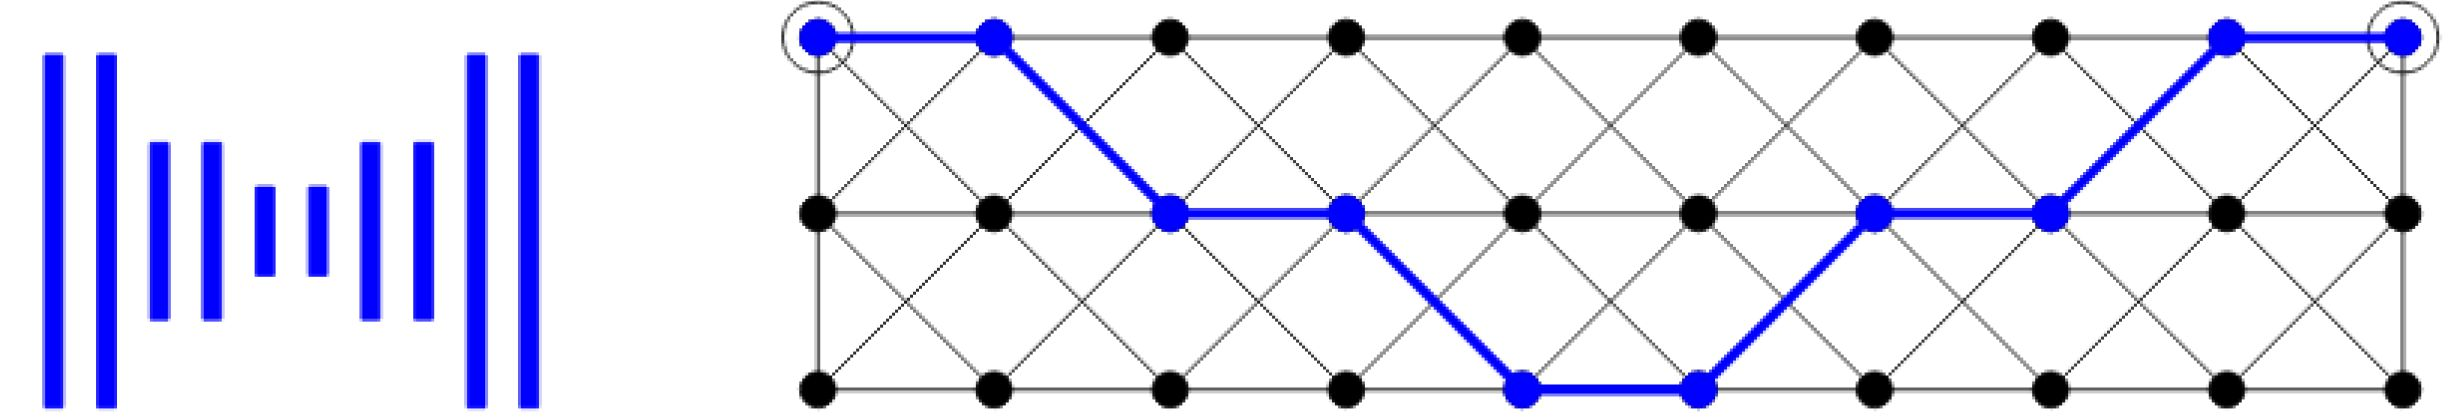
\includegraphics[width=1.02\textwidth]{images/conv_fabric_3.jpg}\vspace*{-0.5cm}}
	
%\only<2>{\bigskip\bigskip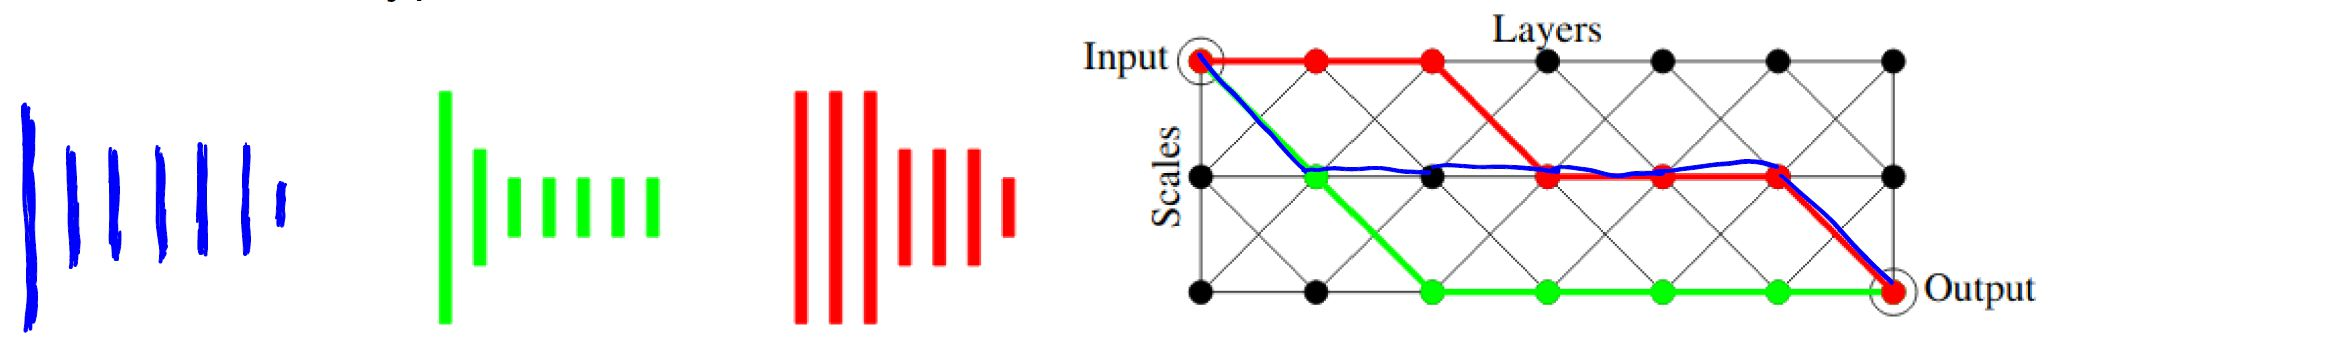
\includegraphics[width=0.7\textwidth]{images/conv_fabric_2.jpg}}
%\pause
%	\medskip
%		\myit{
%			\item \alert{Each path} from the input to the output \alert{represents an architecture}
%	\pause
%	\smallskip
%			\item The \alert{nodes represent tensors}
%			\item The \alert{edges represent computations} (e.g., convolution / strided convolution)
%	\pause
%	\smallskip
%		\item \alert{Weights for the operation on an edge are shared}\\ across all (exponentially many) architectures that have that edge
%		}
	}
%\pause
%\bigskip
	%\centering
	\only<2-5>{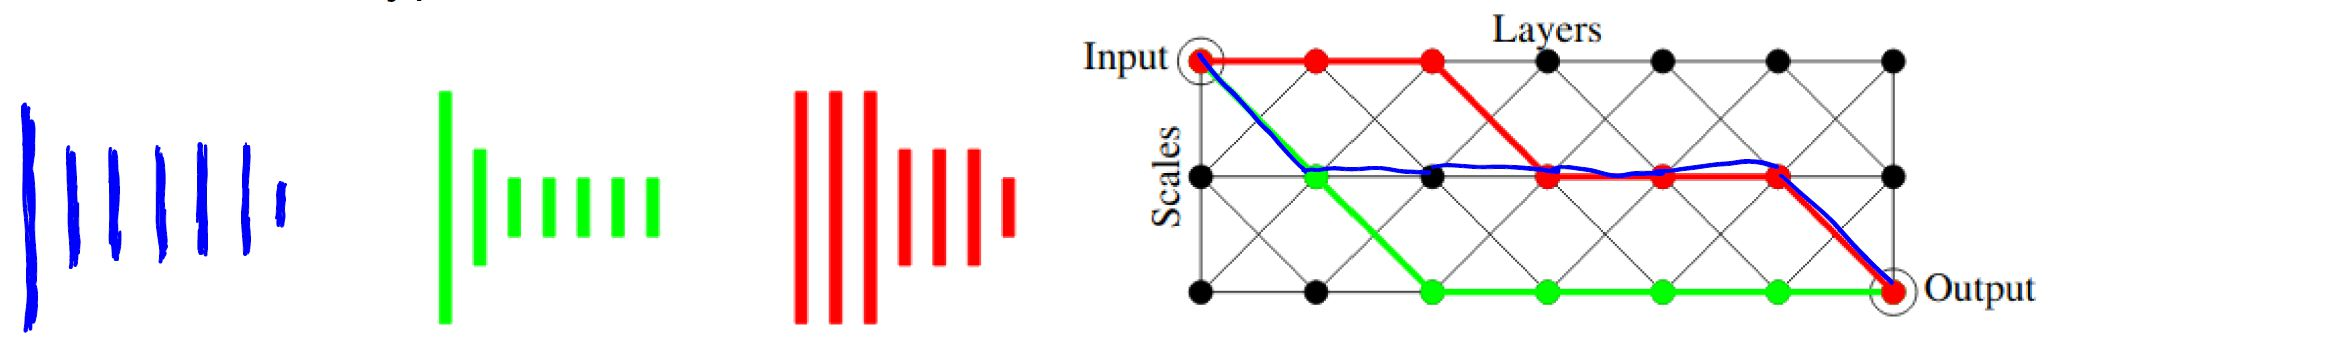
\includegraphics[ scale= 1, width= 15.24cm]{images/conv_fabric_2.jpg}}
	 
}
%----------------------------------------------------------------------

%-----------------------------------------------------------------------
\myframetop{One-shot models for cell search spaces}{

\vspace*{-0.2cm}
\myit{
	\item \alert{Directed acyclic multigraph} to capture all (exponentially many) cell architectures		
		\myit{
			\item The \alert{nodes represent tensors}
			\item The \alert{edges represent computations} (e.g., 3x3 conv, 5x5 conv, max pool, \ldots)
			\item The results of operations on multiple edges between two nodes are combined (addition/concatenation) 
		}
\bigskip
\visible<2->{
	\item Individual architectures are subgraphs of this multigraph
	\myit{
		\item \alert{Weights for the operation on an edge are shared}\\ across all (exponentially many) architectures that have that edge
	}		
}
%	\item This one-shot model is \alert{trained as a standard neural network} with mini-batches and stochastic optimizers.
%	\visible<2->{\item At each mini-batch iteration \alert{weights are shared} between different architectures with common edges/nodes in the supergraph}
	}
\medskip	
	\centering
	\visible<1->{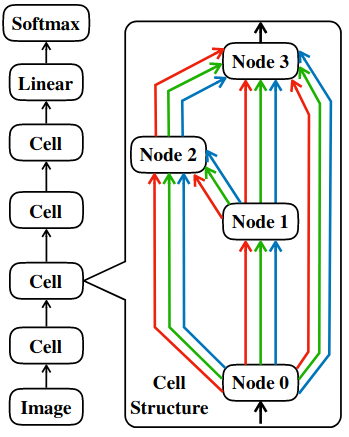
\includegraphics[width=0.19\textwidth]{images/one_shot_model_1.png}\quad\quad\quad\quad\quad\quad}
	\visible<2->{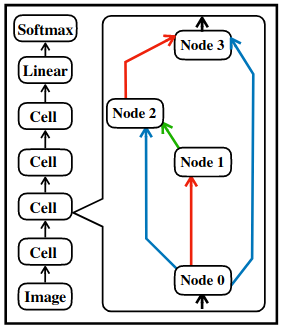
\includegraphics[width=0.19\textwidth]{images/one_shot_model_2.png}\quad\quad}
	\visible<2->{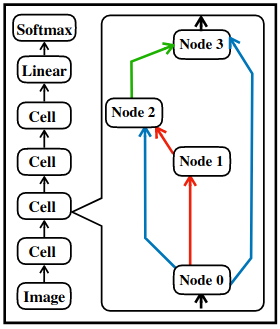
\includegraphics[width=0.19\textwidth]{images/one_shot_model_3.png}}

}
%----------------------------------------------------------------------

%-----------------------------------------------------------------------
%\myframetop{Basic Principle}{
%	\centering
%	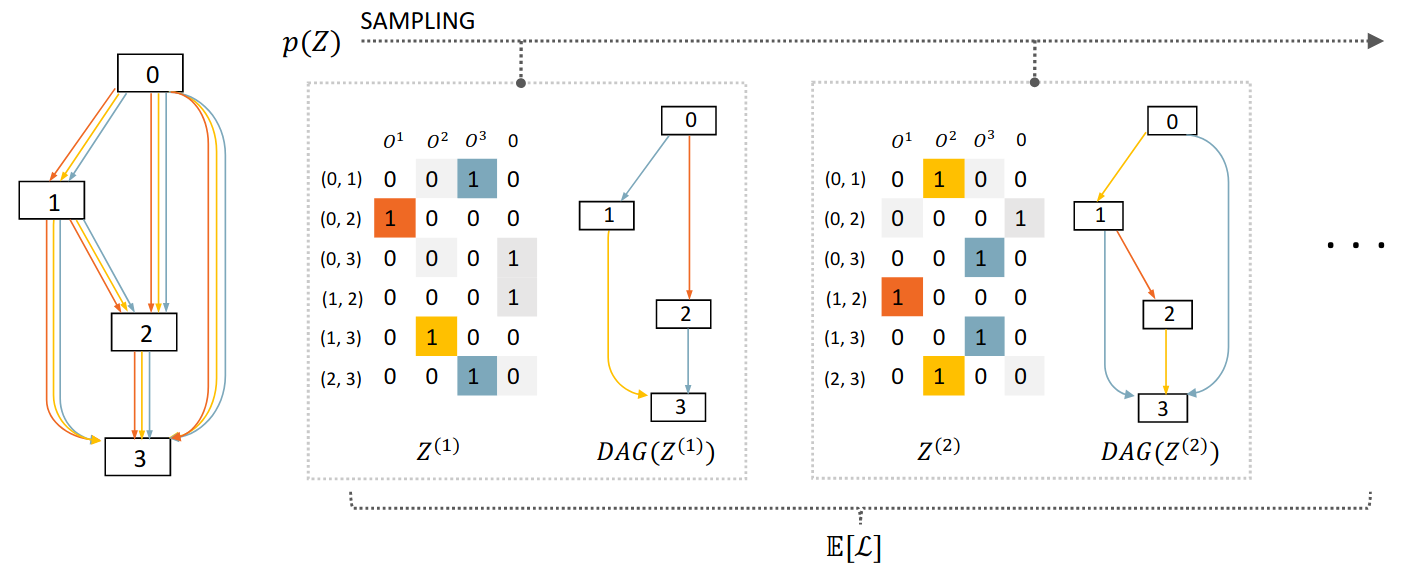
\includegraphics[width=0.7\textwidth]{images/snas_oneshot.png}
%	
%	\only<1>{
%	\begin{itemize}
%	\footnotesize
%		\item The \textbf{one-shot model} is a multi-graph containing all possible DAGs
%		\myit{
%		\footnotesize
%			\item[-] Every DAG represents a single architecture $Z^{(\cdot)}$ in the search space $\mathcal{A}$.
%			\item[-] Nodes represent aggregating operations (e.g. summation, concatenation) for incoming tensors.
%			\item[-] Edges represent operations $O^i$ (in the figure: one color per operation)
%			}
%		\item The row labels in the matrix above represent a pair of nodes $(j,k)$ in the graph and the column labels the operations $O^i$. A value of $1$ means that that operaration is active in the edge connecting node $j$ to $k$.
%	\end{itemize}
%	}
%
%	\only<2>{
%	\begin{itemize}
%	\footnotesize
%		\item The most important principle in one-shot models is \textbf{weight-sharing} between graphs.
%		\myit{
%		\footnotesize
%			\item[-] The one-shot model is trained as a normal neural network, i.e. with mini-batch training. The question is how to distinguish single architectures in the one-shot model during this training?
%			\item[-] One way is that for each sampled mini-batch also sample stochastically an architecture (DAG) and update only the parameters of that architecture.
%			\item[-] For all subsequent iterations in case a new sampled architecture has common edges (i.e. some entries in the matrices are the same) in the DAG, the weights are shared.
%			}
%	\end{itemize}
%	}
%}
%----------------------------------------------------------------------


\myframetop{Training the one-shot model -- standard SGD \litw{\href{https://arxiv.org/pdf/1606.02492.pdf}{Saxena and Verbeek. 2017}}}{

	\myit{
\visible<1->{
		\item One-shot model is an acyclic graph; thus, backpropagation applies
		\myit{
			\item Simplest method: standard training with SGD
			\item This implicitly trains \alert{an exponential number of architectures}
%			\item Used by convolutional neural fabrics		
		}
}
\medskip

%		\myit{
%			\item They did not aim at extracting a strong single architecure
%			\item Rather, they aimed for a good ensemble
%		}
%\pause
%\medskip
\visible<2->{
		\item Potential issue: co-adaptation of weights
		\myit{
			\item Weights are implicitly optimized to work well on average across all architectures
			\item They are \alert{not} optimized specifically for the top-performing architecture
		}
}
	}
\bigskip
	\centering
	\visible<1->{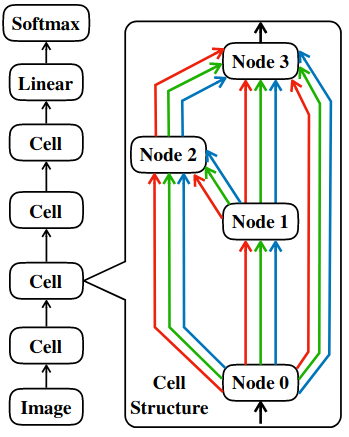
\includegraphics[width=0.2\textwidth]{images/one_shot_model_1.png}}
}
%----------------------------------------------------------------------

%----------------------------------------------------------------------

%\myframetop{Impact of DropPath \litw{\href{http://proceedings.mlr.press/v80/bender18a/bender18a.pdf}{Bender et al., 2018}}}{
%	\centering
%	
%	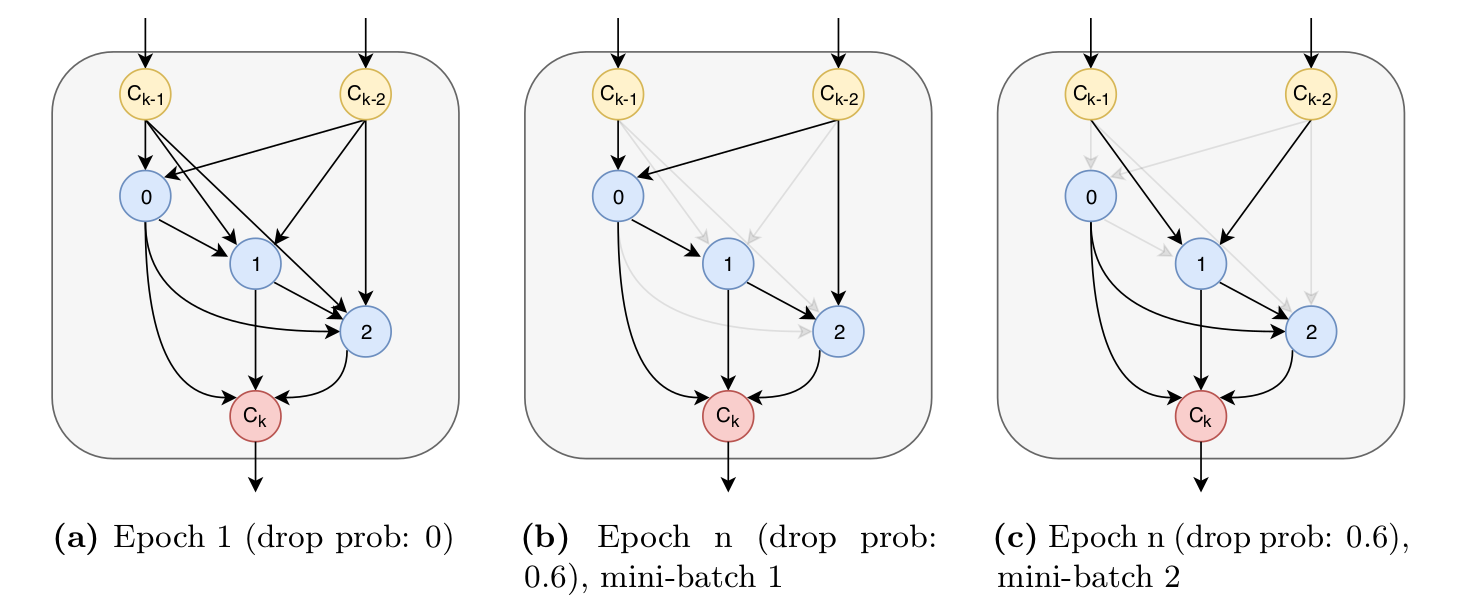
\includegraphics[width=0.8\textwidth]{images/droppath.png}
%	
%    \begin{itemize}
%		\item DropPath zeros out one a subset of the operations at each mini-batch training iteration with probability $p$.
%		\item ScheduledDropPath starts with $p=0$ and increases that linearly throughout training until a maximum $p_{max}$ in the end.
%	\end{itemize}
%}
%---------------------------------------------------------------



%----------------------------------------------------------------------
\myframetop{Training the one-shot model -- DropPath \litw{\href{http://proceedings.mlr.press/v80/bender18a/bender18a.pdf}{Bender et al. 2018}}}{
	\centering
	
	\begin{itemize}
	%\footnotesize
		\item To avoid coadaptation of weights, we can use \alert{DropPath}, a technique analogous to Dropout \lit{\href{https://jmlr.org/papers/volume15/srivastava14a/srivastava14a.pdf}{Srivastava et al. 2014}}:
		\myit{
\visible<2->{
			\item[-] At each mini-batch iteration:\\ for each operation connecting 2 nodes, zero it out with probability $p$
}
\smallskip
\visible<3->{
			\item[-] \alert{ScheduledDropPath}: starts with $p=0$ and increases $p$ linearly to $p_{max}$ at the end of training
}
			}
	\end{itemize}
	
\vspace*{-0.5cm}
\begin{columns}
	\column{0.01\textwidth}
	\column{0.33\textwidth}
	
	\begin{center}
	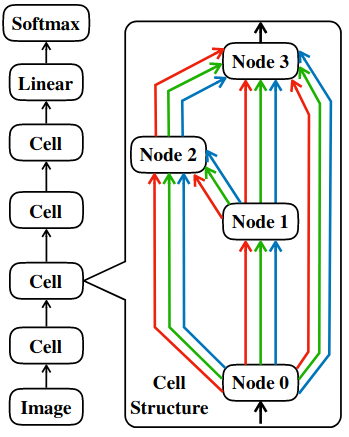
\includegraphics[width=0.6\textwidth]{images/one_shot_model_1.png}\\
	One-shot model
	\end{center}
	
	\column{0.02\textwidth}
	\column{0.33\textwidth}	
	\begin{center}
\visible<2->{	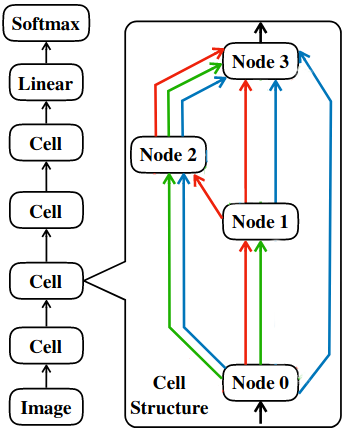
\includegraphics[width=0.6\textwidth]{images/drop_path_1.png}\\
	Architecture for batch 1
}
	\end{center}
	
	\column{0.33\textwidth}	
	\begin{center}
\visible<2->{
	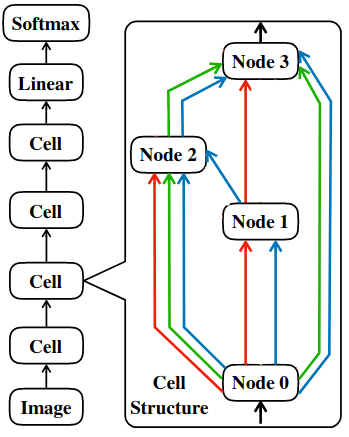
\includegraphics[width=0.6\textwidth]{images/drop_path_2.png}\\
	Architecture for batch 2
}
	\end{center}	

	\column{0.02\textwidth}	
\end{columns}
%	
%	\only<1->{
%	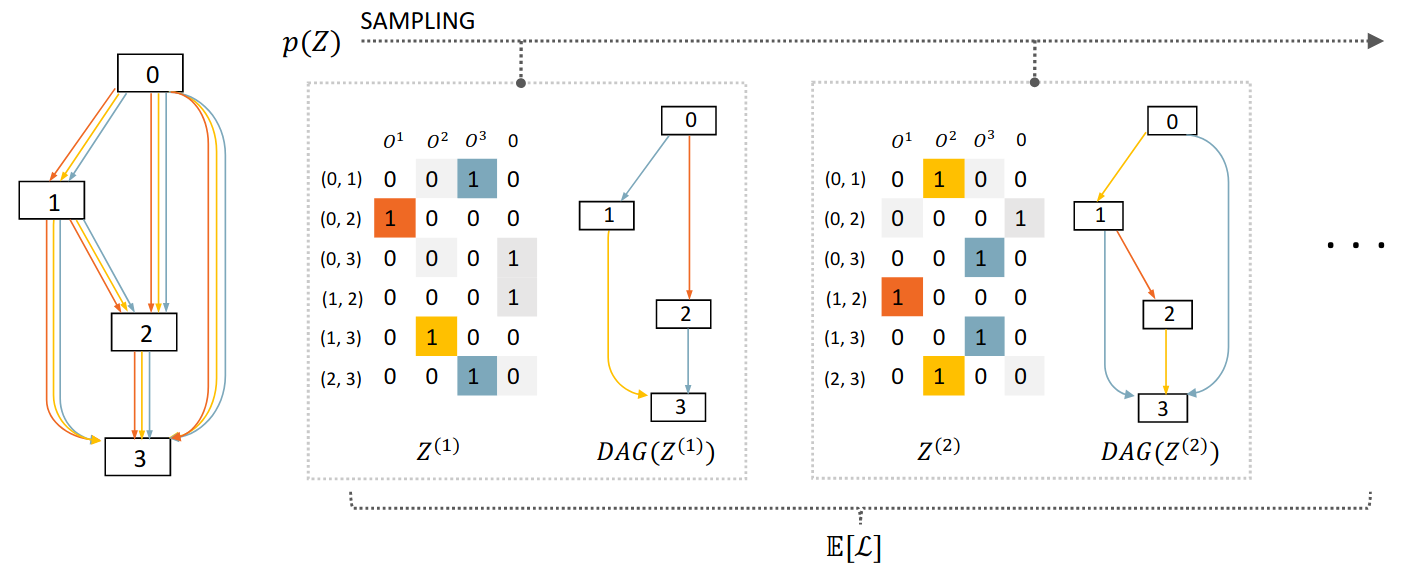
\includegraphics[width=.75\textwidth]{images/snas_oneshot.png}
%	}
}
%---------------------------------------------------------------


%----------------------------------------------------------------------
\myframetop{Training the one-shot model -- Sampling}{
	\centering
	
    \begin{itemize}
		\item At each mini-batch iteration during the training of the one-shot model \alert{sample a single architecture} 
		%$Z$ 
		from the search space 
		%$\mathcal{A}$.
		\visible<3->{
		\myit{
			\item[-] \textbf{Random Search with Weight Sharing} \lit{\href{https://arxiv.org/pdf/1902.07638.pdf}{Li and Talwalkar. 2020}} $\longrightarrow$ sample from uniform distribution
			\item[-] \textbf{ENAS} \lit{\href{https://arxiv.org/pdf/1802.03268.pdf}{Pham et al. 2018}} $\longrightarrow$ sample from the learned policy of a RNN controller
		}
		}
\pause
\medskip
		\item \alert{Update the parameters of the one-shot model} corresponding to only that architecture
	\end{itemize}
	
\vspace*{-0.5cm}
\begin{columns}
	\column{0.01\textwidth}
	\column{0.33\textwidth}
	
	\begin{center}
	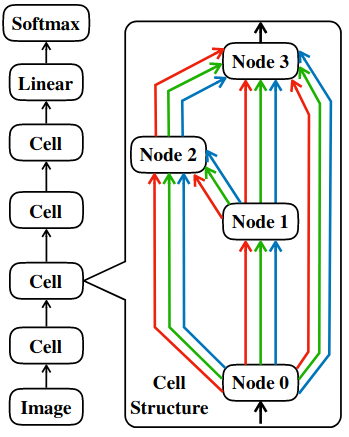
\includegraphics[width=0.6\textwidth]{images/one_shot_model_1.png}\\
	One-shot model
	\end{center}
	
	\column{0.02\textwidth}
	\column{0.33\textwidth}	
	\begin{center}
	\smallskip
	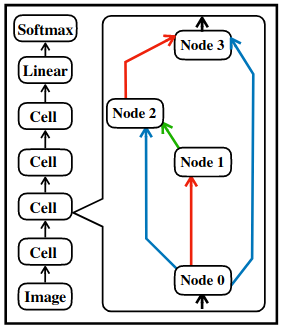
\includegraphics[width=0.6\textwidth]{images/one_shot_model_2.png}\\
	Architecture for batch 1
	\end{center}
	
	\column{0.33\textwidth}	
	\begin{center}
	\smallskip
	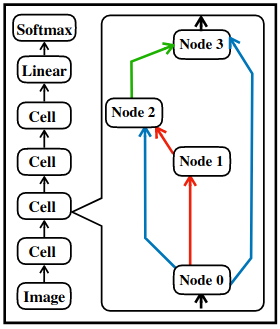
\includegraphics[width=0.6\textwidth]{images/one_shot_model_3.png}\\
	Architecture for batch 2
	\end{center}	

	\column{0.02\textwidth}	
\end{columns}
%	
%	\only<1->{
%	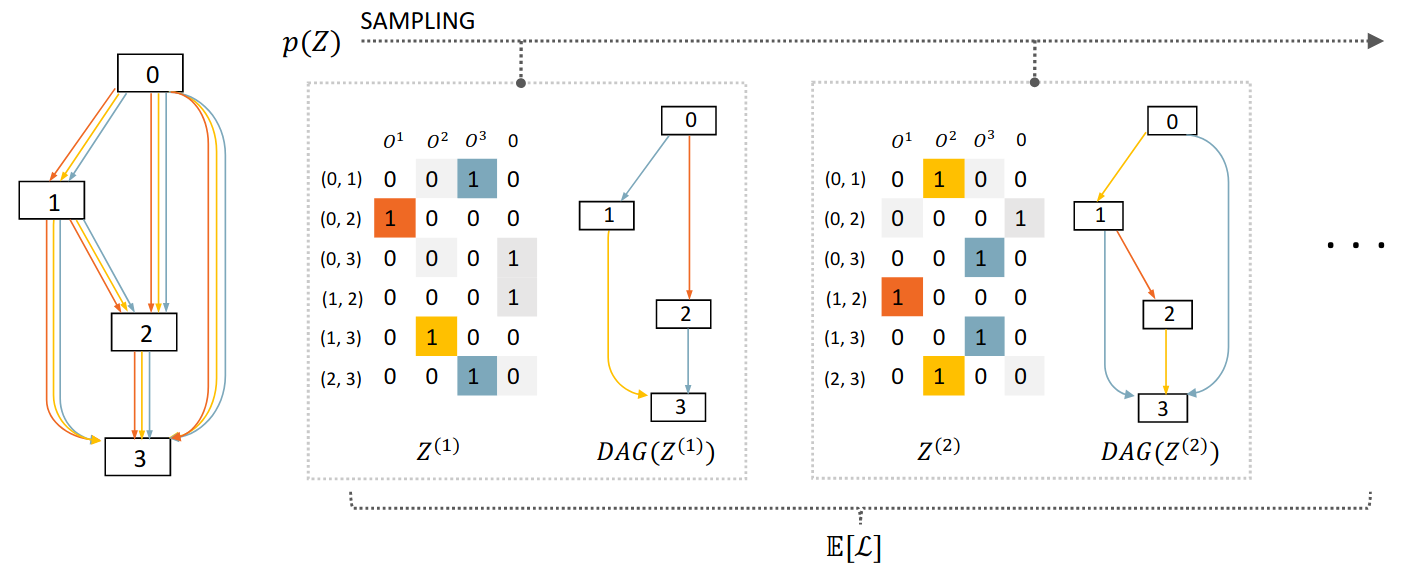
\includegraphics[width=.75\textwidth]{images/snas_oneshot.png}
%	}
}
%---------------------------------------------------------------


%----------------------------------------------------------------------

%\myframetop{Random Search with Weight Sharing \litw{\href{https://arxiv.org/pdf/1902.07638.pdf}{Li and Talwalkar, 2020}}}{
%	\centering
	
%    \begin{itemize}
%		\item Random Search with Weight Sharing \textbf{utilizes the one-shot model to speed up vanilla random search} as follows:
%		\myit{
%			\only<1>{
%			\item[-] At each mini-batch iteration during the training of the one-shot model \alert{sample uniformly at random} one architecture $Z$ from the search space $\mathcal{A}$.
%			\item[-] \alert{Update the parameters of the one-shot model} corresponding to only that architecture.
%			\item[-] After training the one-shot model finishes, sample uniformly at random $M$ architectures and rank them based on the error on a single mini-batch from the validation set \alert{using the one-shot model parameters} (retraining from scratch is computationaly expensive).
%			\item[-] Select the top $K$, where $K < M$, and evaluate those on the full validation set, again using the one-shot parameters.
%			\item[-] Return the top performing architecture to \alert{retrain from scratch}.
%			}
%			\only<2>{
%			\item[-] Works \alert{comparably to state-of-the-art NAS methods} on many benchmarks.
%			}
%		}
%	\end{itemize}
%	
%	\only<2>{
%	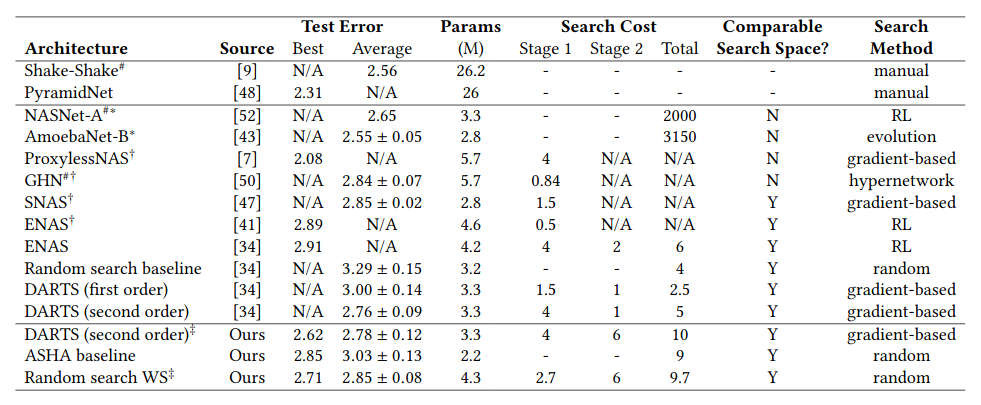
\includegraphics[width=.75\textwidth]{images/rs_ws.png}
%	}
%}
%---------------------------------------------------------------

\myframetop{How to utilize the trained one-shot model?}{
	\centering
	
    \begin{itemize}
		\item After training the one-shot model we have to \alert{select the best individual architecture} from it
		\item There are multiple ways one can approach this. Some of these are:
		\myit{
\pause
			\item[$1$.] Sample uniformly at random $M$ architectures and rank them based on their validation error \alert{using the one-shot model parameters} 
			%(retraining from scratch is computationaly expensive)
			%\item[-] Select the top $K$, where $K < M$, and evaluate those on the full validation set, again using the one-shot parameters.
\pause
			\item[$1b$.] (Optional) Select top $K$ ($K<M$) and retrain them from scratch for a couple of epochs
\pause
			\item[$2$.] Return the top performing architecture to \alert{retrain from scratch} for longer
		}
	\end{itemize}
	
	\onslide<5>{
    	\begin{minipage}{0.4\textwidth}
        	\begin{itemize}
				\footnotesize
				\item \textbf{Pitfall:} the correlation between architectures evaluated with the one-shot weights and retrained from scratch (stand-alone models) should be high
				\item If not, \textbf{selecting the best architecture based on the one-shot weights} is sub-optimal.
			\end{itemize}
	    \end{minipage}
	    \hspace{1cm}
    	\begin{minipage}{0.5\textwidth}
\begin{center}
	        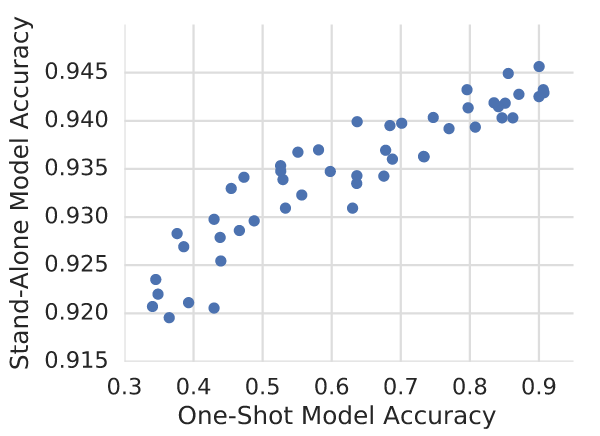
\includegraphics[width=.7\textwidth]{images/bender_correlation_1.png}\\
	        \scriptsize{From \smaller{\lit{\href{http://proceedings.mlr.press/v80/bender18a/bender18a.pdf}{Bender et al. 2018}}}}
\end{center}
    	\end{minipage}
	}
}
%---------------------------------------------------------------

%----------------------------------------------------------------------
\myframe{Questions to Answer for Yourself / Discuss with Friends}{

	\myit{
		\item Repetition:\\ \alert{How are the weights shared in the one-shot model?}
\bigskip
		\item Repetition:\\ \alert{What is the difference between Random Search with Weight Sharing and ENAS?}
\medskip
		\item Discussion:\\ \alert{What migth be some downsides of using the one-shot model for NAS?}
	}	 
}
\end{document}
%-----------------------------------------------------------------------

